\chapter{Grundlagen}

In diesem Kapitel werden die Grundlagen, welche für das weitere Verständnis der Arbeit und der gesamten Anwendung notwendig sind, näher beschrieben. Zunächst werden die verschiedenen Technologien und Frameworks, sowohl des Frontends, als auch des Backends dargestellt. Anschließend werden einige gängige Angriffstypen im \ac{WWW} erläutert.

\section{Frontend Technologien und Frameworks}

Dieser Abschnitt behandelt diejenigen Technologien, die die Interaktion des Benutzers visualisieren. Da es sich bei webifier um eine Webanwendung handelt, sind dies ausschließlich Webtechnologien, welche von grafischen Browsern unterstützt werden.

Die grundlegende Informationssprache des \ac{WWW} heißt \ac{HTML}. Sie wurde ursprünglich entwickelt um wissenschaftliche Dokumente semantisch zu beschreiben (engl. 'to mark up').
Heute wird sie jedoch in weitaus größerem Umfang genutzt.\footcite[Vgl.][]{html5Spec}
\ac{HTML}-Dateien bestehen aus zwei Arten von Informationen: Textdaten und Markupinformationen.
Erstere sind verantwortlich für den textuellen Inhalt der Webseite. Dazu zählen alle abgebildeten Texte wie sie auch in Überschriften, Abschnitten, Menüs, usw. stehen. Sie sind die Informationen, die Betrachter der Webseite direkt über das grafische Browserfenster lesen kann.
Markupinformationen hingegen definieren den Aufbau und die Semantik der Inhalte. Diese sind für den normalen Betrachter nicht unbedingt sichtbar. Hierbei handelt es sich um sogenannte \textit{Tags}, die im Quellcode in spitzen Klammern stehen und aus einer Menge von bestimmten Werten stammen. Tags treten immer in Paaren auf, wobei der zweite Tag (Endtag) zusätzlich einen Backslash zwischen aufgehender spitzer Klammer und Tagnamen hat (s. z.B. \autoref{lst:Beispiel.html} Zeile 5, 10, 11).
Innerhalb dieser beiden Tags können wiederum neue Tags (Zeile ), aber auch einfache Textdaten stehen (s. Zeilen 4, 7, 8, 9).
Diese Verschachtelung führt dazu, dass meist ein komplexer Baum von Tagelementen entsteht. Zu den wichtigsten Tags zählt der \lstinline{<html>}-Tag. Er ist der äußerste Wurzeltag, der alle anderen Tags umschließt. Der \lstinline{<head>}- und \lstinline{<body>}-Tag stehen beide eine Ebene tiefer und beinhalten Metadaten für das gesamte Dokument bzw. den Seiteninhalt.\footcite[Vgl.][57]{webTechnologies}

\begin{scriptsize}
\lstset{
    style=eclipsehtml,
    caption={Beispiel.html},
    label={lst:Beispiel.html}
}
\begin{lstlisting}
<!DOCTYPE html>
<html>
<head>
	<title>Testseite</title>
</head>
<body>
	<h1>Überschrift</h1>
	<p>Abschnitt 1</p>
	<p>Abschnitt 2</p>
</body>
</html>
\end{lstlisting}
\end{scriptsize}

\todo[color=cyan]{Daniel schreiben: \ac{CSS}}

\label{javascript}
\todo[color=cyan]{Daniel schreiben: JavaScript}
\todo[color=cyan]{Daniel schreiben: jQuery}
\todo[color=cyan]{Daniel schreiben: Bootstrap}

\section{Backend Technologien und Frameworks}

In diesem Abschnitt werden nun alle Technologien und Frameworks vorgestellt welche in den Backends der einzelnen Teilanwendungen zum Einsatz kamen.

Wohl am häufigsten kam die Programmiersprache Java zum Einsatz. Java ist eine universal einsetzbare, nebenläufige, klassenbarierte und objektorientierte Programmiersprache. Sie wurde möglichst einfach gestaltet um von vielen Entwicklern genutzt zu werden. In ihrer Syntax ähnelt sie den Programmiersprachen C und C++. Außerdem ist sie stark und statisch typisiert. Vorallem aber zeichnet sich Java durch seine plattformunabhängigkeit aus. Diese wird dadurch umgesetzt, dass Java-Quellcode in plattformunabhängigen Byte-Code kompiliert wird, welcher von einer \ac{JVM} ausgeführt wird. Java ist eine Hochsprache, die mit Hilfe des so genannten \enquote{Garbage Collectors} eine automatische Speicherverwaltung bereitstellt. \footcite[Vgl.][1]{javaspecification}

In einigen Teilprojekten wurde das auf Java basierende \textit{Spring}-Framework verwendet. \textit{Spring} stellt eine vereinfachte Möglichkeit auf den Zugriff auf viele \ac{API} der Standard-Version zur Verfügung. Ein weiterer wesentlicher Bestandteil des \textit{Spring}-Frameworks ist die \textit{Dependency Injection}. Hierbei suchen sich Objekte ihre Referenzen nicht selbst, sondern bekommen diese Anhand einer Konfiguration injiziert. Dadurch sind sie eigenständig und können in verschiedenen Umgebungen eingesetzt werden. Des weiteren bringt \textit{Spring} eine Unterstützung für aspektorientierte Programmierung mit, wodurch mit verschiedenen Abstraktionsschichten einzelne Module abgekapselt werden können. \footcite[Vgl.][2]{spring3}

Aufbauend auf dem \textit{Spring} Basis-Modul werden noch weitere Module, wie beispielsweise Spring Security, Sprint Boot, Spring Integration, Spring Data, Spring Session oder Spring MVC. \footcite[Vgl.][2]{springPivotal} Im folgenden werden die \textit{Spring}-Mudule naäher erläutert, die für das weitere Verständnis der Arbeit notwendig sind.

\begin{description}
  \item[Spring Boot] \hfill \\
    Mit Spring Boot können Anwendungen, welche das \textit{Spring}-Framework nutzen, einfacher eintwickelt und ausgeführt werden, da dadurch eigenständig lauffähige Programme erzeugt werden können, welche nicht von externen Services abhängig sind. Hierfür bringt Spring Boot einen Integrierten Server mit, auf welchem die Anwendung bereitgestellt wird.\footcite[Vgl.][1]{springBoot}
  \item[Spring MVC] \hfill \\
    Spring MVC ist sehr gut geeignet um Webanwendungen zu implementieren.\footcite[Vgl.][3]{spring3} Hierfür können die diese in mehrere Abstraktionsschichten gegliedert werden. Beispielsweise in das \ac{UI}, die Geschäftslogik und die Persistenzschicht.\footcite[Vgl.][21]{springMvc}
  \item[Spring Data] \hfill \\
    Spring Data vereinfacht Datenbankzugriffe ungemein. Das Modul stelt \ac{API}s für fast alle gängigen Datenbankzugriffsschichten, wie JDBC (Java Database Connectivity), Hibernate, JDO (Java Data Objects) zur Verfügung. Aber nicht nur relationale Datenbanken werden unterstützt, sondern beispielsweise auch NoSQL-Datenbanken und Key/Value-Stores können Problemlos eingesetzt werden.\footcite[Vgl.][3f]{springData}
\end{description}

In Verbindung mit Spring Data wurde eine \textit{MongoDB} zur Speicherung der Ergebnisse eingesetzt. \textit{MongoDB} ist eine Dokument orientierte anpassungsfähige und skalierbare Datenbank. Sie vereint viele nützliche Eigenschaften von Relationalen Datenbanken, wie Sekundärindizes, Auswahlabfragen und Sortierung mit Skalierbarkeit, MapReduce-Aggregationen und raumbezogenen Indizes. Außerdem gibt es bei MongoDB keine festen Schemata, weshalb großen Datenmigrationen normal nicht notwendig sind.\footcite[Vgl.][1f]{mongodb}

Gewonnene und gespeicherte Daten müssen danach auch noch aufbereitet und visualisiert werden. Webifier setzt dafür auf die Programmiersprache R. R ist eine freie Programmiersprache, entwickelt für statistische Auswertungen und Visualisierungen. Sie zählt zu den prozeduralen Programmiersprachen. Die quelltextoffene Programmiersprache wird ständig weiterentwickelt. Zusätzlich gibt es eine Vielzahl an Packages, welche weitere Funktionalität bereitstellen. Diese sind über ein zentrales Repository abrufbar und so leicht einbindbar in den Quelltext. \footcite[Vgl.][1ff]{R}

Ein wichtiger Bestandteil jedes großen Software-Projektes ist ein gutes Build-Management-Tool. Für webifier wurde \textit{Gradle} als solches gewählt. Ein Build-Prozess besteht grundsätzlich aus zwei Teilschritten. Zum Einen aus dem kompilieren des Codes und zum anderen aus dem verlinkten der benutzen Bibliotheken. \footcite[Vgl.][]{buildprozess}
Da das manuelle Einbinden von Bibliotheken und compilieren des Codes bei großen Projekten sehr aufwändig und mühsam sein kann wird hier auf Build-Management-Tools wie \textit{Gradle} zurückgegriffen. Um den Build für den Nutzer möglichst einfach zu gestalten verfolgt Gradle zwei Prinzipien. Das erste Prinzip ist \textit{Convention over Configuration}, was bedeutet, dass soweit es geht ein Standardbuildprozess definiert ist und der Anwender nur die Parameter ändern muss die Projektspezifisch abweichen. Das zweite Prinzip nennt sich \ac{DRY}. Hierbei geht es darum Redundanzen in der Konfiguration des Buildes zu vermeiden. Diese beiden Prinzipien helfen Gradle, dass meist kurze Build-Skripte ausreichen um komplexe Prozesse abzubilden. \footcite[Vgl.][6f]{gradle}

Die Kommunikation zwischen Server und Client erfolgt über \ac{REST}. Hierbei wird jedes Objekt in \ac{REST} als Ressource definiert, welche über einen eindeutigen \ac{URI} adressiert werden können. Über die HTTP-Methoden GET, PUT, POST und DELETE können diese Ressourcen geladen, erstellt, geändert oder auch gelöscht werden. \footcite[Vgl.][]{rest}

Das Testen von potenziell gefährlichen Webseiten soll natürlich nicht direkt auf dem Server geschehen, da es sonst diesen potenziell gefährden könnte. Deshalb wird hierfür eine Virtualisierung benötigt um die Tests abgekapselt vom Gesamtsystem auszuführen. Dafür wurde Docker als Tool eingesetzt. Docker ist eine Open-Source-Software zur Virtualisierung von Anwendungen. Hierbei wird auf die Container-Technologie gesetzt. Container sind vom Betriebssystem bereitgestellte virtuelle Umgebung zur isolierten Ausführung von Prozessen. Ein Vorteil der Container gegenüber der herkömmlicher virtuelle Maschinen ist der vielfach geringere Ressourcenbedarf.\footcite[Vgl.][]{docker}

\section{Technologien und Frameworks der Tests}

In diesem Kapitel werden diejenigen Technologien und Frameworks erläutert, die zur Umsetzung der Sicherheitstests verwendet werden.

\todo[color=cyan]{Daniel schreiben: Python}
Python ist eine Programmiersprache, die einen schnellen Projektstart ermöglicht und ist auf Integration von verschiedenen Systemen spezialisiert.
Die Sprache wird von der Python Software Foundation nach Open Source Standards entwickelt.
Die aktuellste Version ist Python 3.6.1, wobei bei der Implementierung der Tests keine einheitliche Version verwendet wird\todo{diesen Nebensatz in Retrospektive, als Punkt zur Verbesserung?}.
Python zählt zu den dynamisch typisierten Programmiersprachen, was bedeutet, das es wie bei JavaScript\ref{javascript} erst zur Laufzeit zu einer Typenprüfung kommt.
Weiterhin werden Codeblöcke nicht durch Sonderzeichen (wie z.B. geschweifte Klammern in Java) gekennzeichnet, sondern definieren sich an der Einrückungstiefe.
\footcite{pythonHomepage}
%Deshalb verwenden sechs von neun Tests Python.

\todo[color=cyan]{Daniel schreiben: Phantom JS}

Um Webseiten mit allen ihren Ressourcen herunterzuladen wurde die freie Software \textit{HTTrack} verwendet. Mit \textit{HTTrack} können Webseiten in einem lokalen Verzeichnis gespeichert werden. Hierfür erzeugt das Programm rekursiv alle notwendigen Verzeichnisse und läd anschließend alle Ressourcen, wie \ac{HTML}-, \ac{CSS}- und JavaScript-Dateien, als auch Bilder und andere Dateien herunter. Außerdem ist es möglich automatisiert alle \ac{HTML}-Links entsprechend zu modifizieren. Abschließend bietet HTTrack umfassende Konfigurationsoptionen um es für den optimalen Gebrauch anpassen zu können.\footcite[Vgl.][]{httrack}

Für die Analyse und den Vergleich von Bildern wurde auf die freie JavaScript-Bibliothek Resemble.js zurückgegriffen. Mit Resemble können jegliche Arten von Bildanalyse und Bildvergleich genutzt werden. Urspünglich wurde es für eine Bibliothek von Phanton JS entwickelt, kann aber inzwischen vielseitig eingesetzt werden. Resemble bietet einige Einstellungsmöglichkeiten um Bilder analysieren und miteinander vergleichen zu können. Als Resultat liefert es bei der Bildanalyse Helligkeits- und Farbwerte des Bildes. Beim Bildvergleich bekommt man den prozentualen Unterschied der beiden Bilder, sowie einige zusatzinformationen. Außerdem ist es möglich mit Resemble.js ein Differenzbild mit der Hervorhebung der Unterschiede zweier Bilder zu erzeugen.\footcite[Vgl.][]{resemblejs}

Zu einer umfassenden Analyse gehört selbstverständlich auch die Analyse des Netzwerktraffics. Dazu wird ein entsprechendes Tool genutzt. Webifier nutzt für diesen Zweck den \textit{Bro Network Security Monitor}. Bro ist ein Unix-basiertes \ac{NIDS}.\footcite[Vgl.][199]{bro} Zudem ermöglicht Bro dem Nutzer den Netzwerktraffic zu loggen und mittels eigener Skriptsprache zu filtern. \footcite{bro2} Die Logging-Möglichkeiten werden für die Analyse des Traffics genutzt um mögliche verdächtige Abfragen zu erkennen.


\section{Angriffstypen}

In diesem Abschnitt werden nun einige übliche Angriffstypen von Webseiten auf den Nutzer vorgestellt und eine mögliche Überprüfung in webifier dargestellt.

\todo{Samuel: Noch allgemeiner auf das Thema eingehen\ldots}

\subsection{Malware}

Spyware, Root Kits, Trojaner und viele mehr - alles das ist Malware, welche den Nutzern in unterschiedlichen Weisen kleineren, oder größeren Schaden zuführen. Kurz: Malware ist Software mit bösartiger Wirkung. In diesem Abschnitt werden nun einige Formen von Schadsoftware beschrieben und wie diese in ein System gelangen kann.\footcite[Vgl.][95]{netzwerkDatensicherheit}

Malware ist so vielfältig wie gutartige Anwendungen. Dennoch lässt sie sich auf verschiedene Weisen klassifizieren. Allerdings sind die Wübergänge der einzelnen Klassen fließend. Zum Einen kann Malware im Hinblick auf ihre Verbreitungsmethode und zum Anderen in der Art des Schadens für den ungewollten Anwender unterschieden werden. Alle Klassen vereint jedoch dass Malware im allgemeinen Code enthält, welcher dem Nutzer oder dessen System Schaden zufügt.\footcite[Vgl.][95\psq]{netzwerkDatensicherheit}

Bei der Verbreitungsmethode kann zwischen Viren, Trojanern und Würmern unterschieden werden. Viren sind Programme, welche sich bei der Ausführung selbst kopieren, beispielsweise indem sie ihren Code in andere Programme oder Dokumente des Nutzers einschleusen.\footcite[Vgl.][95]{netzwerkDatensicherheit} Die ersten Viren wurden Anfang der 1980er Jahre in Umlauf gebracht, allerdings spielten Viren sogar schon 1970 in dem Science Fiction Film \textit{The Scarred Man} eine Rolle.\footcite[Vgl.][14]{virusesMalware} Trojaner sind Anwendungen, welche vortäuschen gutartig zu sein, aber Code beinhalten, welcher dem System oder dem User schadet. Trojaner sind seit 1972 bekannt und verbreiten sich üblicher Weise nicht eigenständig.\footcite[Vgl.][12\psq]{virusesMalware} Würmer verbreiten sich üblicherweise von alleine über Netzwerke und infizieren so andere Systeme. Hierfür nutzen sie Schwachstellen in Netzwerkdiensten und schädigt so der Maschine oder dem Anwender.\footcite[Vgl.][95]{netzwerkDatensicherheit} Die ersten Würmer sind wie die ersten Viren in der Science Fiction zu finden. Würmer kommen in dem Roman \textit{The Shockwave Rider} von John Brunner aus dem Jahr 1975 vor. Die ersten realen Würmer waren bereits 1970 im damalign Arpanet zu finden.\footcite[Vgl.][15]{virusesMalware}

Anhand des angerichteten Schadens kann Malware in Spyware, Adware, Malware-Dialer, Zombie-Malware, Backdoors und Root Kits unterteilt werden. Spyware ist Software, welche ohne Wissen des Nutzers Informationen sammelt und weiterleitet. Dadurch könne vertrauliche Daten gestohlen und missbraucht werden.\footcite[Vgl.][95\psq]{netzwerkDatensicherheit} Solche Daten können beispielsweise Benutzernamen und Passworter, E-Mailadressen, Bankaccounts und Kreditkartennummern oder Softwarelizenzschlüssel sein. Mitte der 1990er Jahre war erste Spyware zu finden.\footcite[Vgl.][16]{virusesMalware} Als Adware werden Programme bezeichnet, welche dem Benutzer Werbeanzeigen einblenden.\footcite[Vgl.][96]{netzwerkDatensicherheit} Adware ist ähnlich zu Spyware, da beide Informationen über den Nutzer sammeln. Allerdings ist Adware mehr auf Marketing fokussiert und nutzt die Informationen um dem Nutzer Webung zu präsentieren.\footcite[Vgl.][17]{virusesMalware} Dialer sind Programme, welche Computern über Modems oder Telefonnetze Zugang zum Internet anbieten. Malware-Dialer nutzen das aus und wählen die Rechner ohne Kentniss des Nutzers in teure Service-Rufnummern oder Anwahlpunkte im Ausland ein. Allerdings findet man diese Art von Malware nur noch selten, da es inzwischen telefonbasierten Internetzugänge an Bedeutung verlieren. Software, welche Rechner komprommitiert, wird als Zombie-Malware bezeichnet, da dieser so von Angreifern ferngesteuert werden kann.\footcite[Vgl.][96]{netzwerkDatensicherheit} Am häufigsten werden Zombie-Rechner eingesetzt um Spam zu versenden oder mit vielen anderen Denial of Service Angriffe auszuführen.\footcite[Vgl.][18]{virusesMalware} Backdoors sind modifizierte Programme des Systems, über welche Hacker Sicherheitsmechanismen umgehen und sich so unbefugten Zugriff auf den Rechner verschaffen kann. Modifizierte Softwaregruppen, welche zum Ziel haben deren Aktivität oder die eines Angreifers vor Systembenutzern, inklusive Administratoren zu verstecken werden als Root Kits bezeichnet.\footcite[Vgl.][96]{netzwerkDatensicherheit}

\begin{figure}[h]
\centerline{%
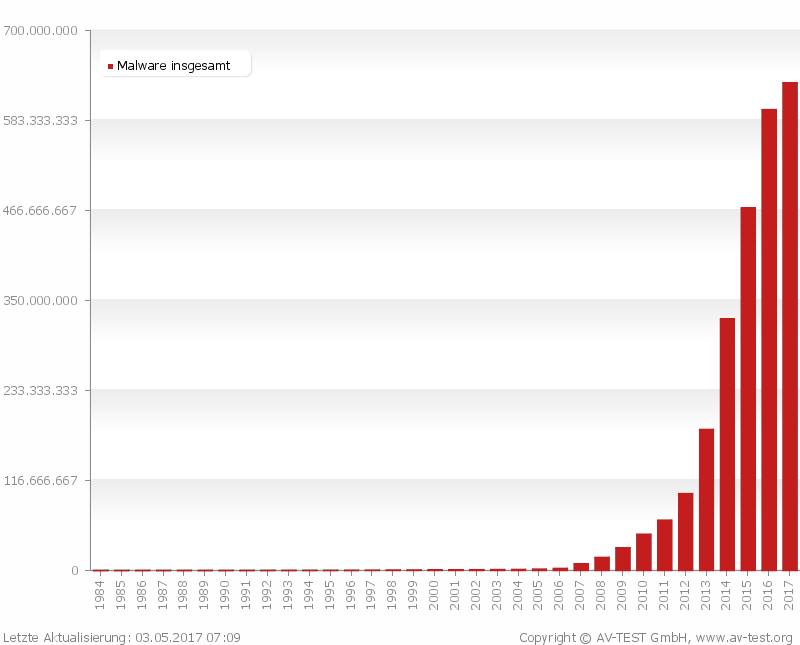
\includegraphics[width=0.5\textwidth]{images/malware-all-years_sum_de}%
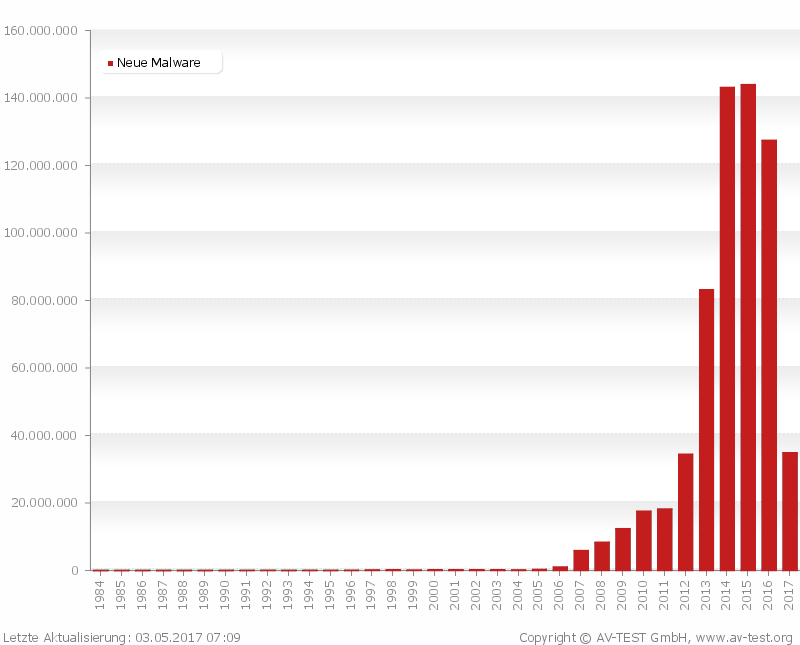
\includegraphics[width=0.5\textwidth]{images/malware-all-years_de}%
}%
\caption{Malware Statistik}
\label{fig:malware-statistics}
\end{figure}

\todo{Statistik einfügen}

Die Verbreitung von Malware beginnt größtenteils über Webseiten und E-Mails.\footcite[Vgl.][97]{netzwerkDatensicherheit} Deshalb ist es notwendig mit webifier Webseiten auf Malware zu prüfen.

\subsection{Request Header Investigation}

\todo[color=cyan]{Daniel schreiben: Request Header Investigation}

\subsection{JavaScript Port Scanning}

\todo{Jani}

\subsection{JavaScript IP Scanning}

\todo{Jani}

\subsection{Clickjacking}

\todo{Jani}

\subsection{Phishing}

Beim Phishing versucht ein Angreifer, in diesem Fall auch Phisher genannt, auf betrügerische Weise vertrauliche oder sensible Anmeldedaten zu bekommen. Um dies zu erreichen gibt fälscht er die elektronische Kommunikation zwischen Opfer und einer vertrauenswürdigen oder öffentlichen Organisation, indem er sich selbst als diese ausgibt. Dies geschieht meist durch E-Mails, welche das Opfer auf eine Webseite locken, welche vermeindlich zur vertrauenswürdigen Organisation gehört, in Wahrheit aber vom Angreifer kontrolliert wird und deshalb Informationen, vorzugsweise Passwörter oder Krefitkartennummern abfängt.\footcite[Vgl.][1]{phishing}

Phishing gibt es seit Anfang der 1990er Jahre, allerdings sind die Zahlen von Phishing-Angriffen in den letzten Jahren drastisch gestiegen. Phishing ist zu einer gefährlichen Kombination aus Social Engeneering und technischen Angriffen geworden, welche zum Ziel hat vertrauliche Informationen zu erlangen. Die gewonnenen Daten werden für Betrug, Identitätsdiebstahl und Spionage missbraucht. \footcite[Vgl.][1\psq]{phishing}

Im Folgenden wird ein beispielhafter Phishingangriff auf PayPal geschildert. PayPal ist ein Online-Bezahldienst mit über 18 Millionen Nutzern alleine in Deutschland. \footcite[Vgl.][]{paypal} Am häufigsten wird PayPal genutzt um Internetkäufe zu bezahlen. Listing \ref{lst:phishing-mail} zeigt eine E-Mail, mit der ein PayPal-Nutzer auf eine Phishing-Seite gelockt werden soll.\footcite[Vgl.][10]{phishing}

\begin{scriptsize}
\lstset{
    style=nonumbers,
    caption=[Phishing Lockmail]{Phishing Lockmail\protect\footnotemark},
    label={lst:phishing-mail}
}
\begin{lstlisting}
Sehr geehrter PayPal-Kunde, sehr geehrte PayPal-Kundin,

wir haben gerade einen oder mehrere Loginversuche von einer fremden IP-Adresse auf Ihr
PayPal-Konto festgestellt.

Wenn Sie in der letzten Zeit unterwegs auf Ihren Account zugegriffen haben, könnten die
ungewöhlichen Loginversuche von Ihnen stammen. Auch wenn die Loginversuche nicht von Ihnen
stammen, besuchen Sie PayPal bitte sobald wie möglich um Ihre Identität zu verifizieren:

(*https://www.paypal.com/signin?country.x=DE&locale.x=de_DE*)

Die Bestätigung Ihrer Identität ist eine Sicherheitsmaßnahme, mit der sichergestellt wird,
dass Sie die enzige Person sind, die Zugriff auf Ihr Konto hat.

Vielen Dank für Ihre Unterstützung um gemeinsam Ihr Konto zu schützen.

Mit freundlichen Grüßen,
PayPal
-------------------------------------------------------------------------
                        SCHÜTZEN SIE IHR PASSWORT

Geben Sie ihr Passwort niemals an Dritte weiter und nutzen Sie es ausschließlich um sich auf
(*https://www.paypal.com/*) anzumelden. Schützen Sie sich vor Betrug, indem Sie einen
neuen Browser öffnen und jedes mal die PayPal Url eintippen um sich anzumelden.
-------------------------------------------------------------------------

Bitte antworten Sie nicht auf diese E-Mail. Nachrichten, die an diese Adresse gesendet werden
können nicht beantwortet werden. Wenn Sie Hilfe benötigen melden Sie sich in Ihrem
PayPal-Konto an und klicken Sie auf den \enquote{Hilfe}-Link im Menü.

PayPal E-Mail ID PP321
\end{lstlisting}
\end{scriptsize}
\footnotetext{\cite{phishing}, S. 11 Abbildung 1.4, Übersetzung Samuel Philipp}

Die in Listing \ref{lst:phishing-mail} dargestellte E-Mail täuscht dem Kontoinhaber vor, dass eine Fremde Person auf das Konto zugegriffen hat und animiert ihn so dazu dem vermeindlich sichern Link zu folgen um seine Identität zu verifizieren um seinen Account zu schützen. Nebenbei sei noch erwähnt, dass der Link in der E-Mail natürlich nicht auf die orginale PayPal-Webseite verweist, sondern auf die Phishing-Seite des Angreifers. Der Hinweiß \enquote{Schützen Sie Ihr Passwort} verleiht der E-Mail noch ein authentischeres Aussehen und würde der Nutzer dem Rat folgen wäre dieser Phishing-Angriff wirkungslos. Viele Nutzer nehmen diesen Rat auch wahr, nutzen aber trotzdem den bereitgestellten Link aus der E-Mail, da diese ja offensichtlich von PayPal stammt und deshalb vertrauenswürdig ist.\footcite[Vgl.][10]{phishing}

Üblicher Weise wird auch die Absenderadresse der E-Mail gefälscht und eine orginaladresse von PayPal, beispielsweise \textit{service@paypal.com} verwendet. Wenn der Empfänger der E-Mail nun den Link aus selbiger öffnet wird er auf die in Abbildung \ref{fig:paypal-phishing-site} dargestellte Webseite geleitet, welche Ihn zur eingabe seiner Anmeldedaten auffordert.\footcite[Vgl.][10]{phishing}

\begin{figure}[H]
  \centering
  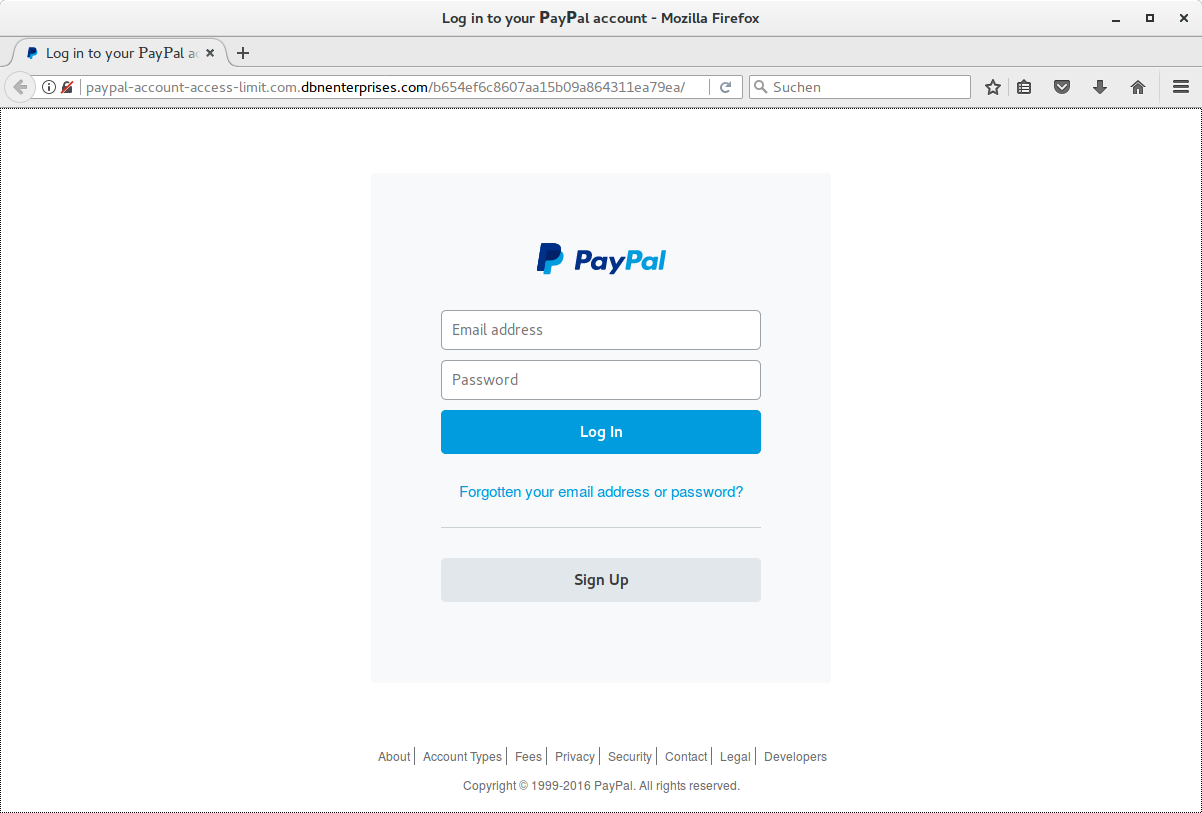
\includegraphics[width=15cm]{images/paypal-phishing-site}
  \caption{PayPal Phishing Webseite}
  \label{fig:paypal-phishing-site}
\end{figure}

Das aussehen der Phishing-Webseite ist dem des Originals (Abbildung \ref{fig:paypal-original-site}) sehr ähnlich. Wenn das Opfer nun seine Benutzernamen und sein Passwort eingegeben hat ist das erste Ziel des Angreifers bereits erreicht, denn er hat gültige Zugangsdaten zu einem PayPal-Account erhalten. Um aber noch mehr Daten zu bekommen und dem Opfer den Angriff weiterhin zu verschleiern wird der Nutzer in vielen Fällen auf einer nachfolgenden Seite gebeten auch noch seine Anschrift und Kreditkartendaten zu bestätigen, indem er diese auch noch eingeben muss. Danach wird der Nutzer wieder \enquote{abgemeldet} und anschließend auf die orginale PayPal-Webseite (Abbildung \ref{fig:paypal-original-site}) weitergeleitet. Damit ist der Phishing-Angriff abgeschlossen und der Angreifer wird keine Zeit verlieren die Daten zu missbrauchen.\footcite[Vgl.][10\psqq]{phishing}

\begin{figure}[H]
  \centering
  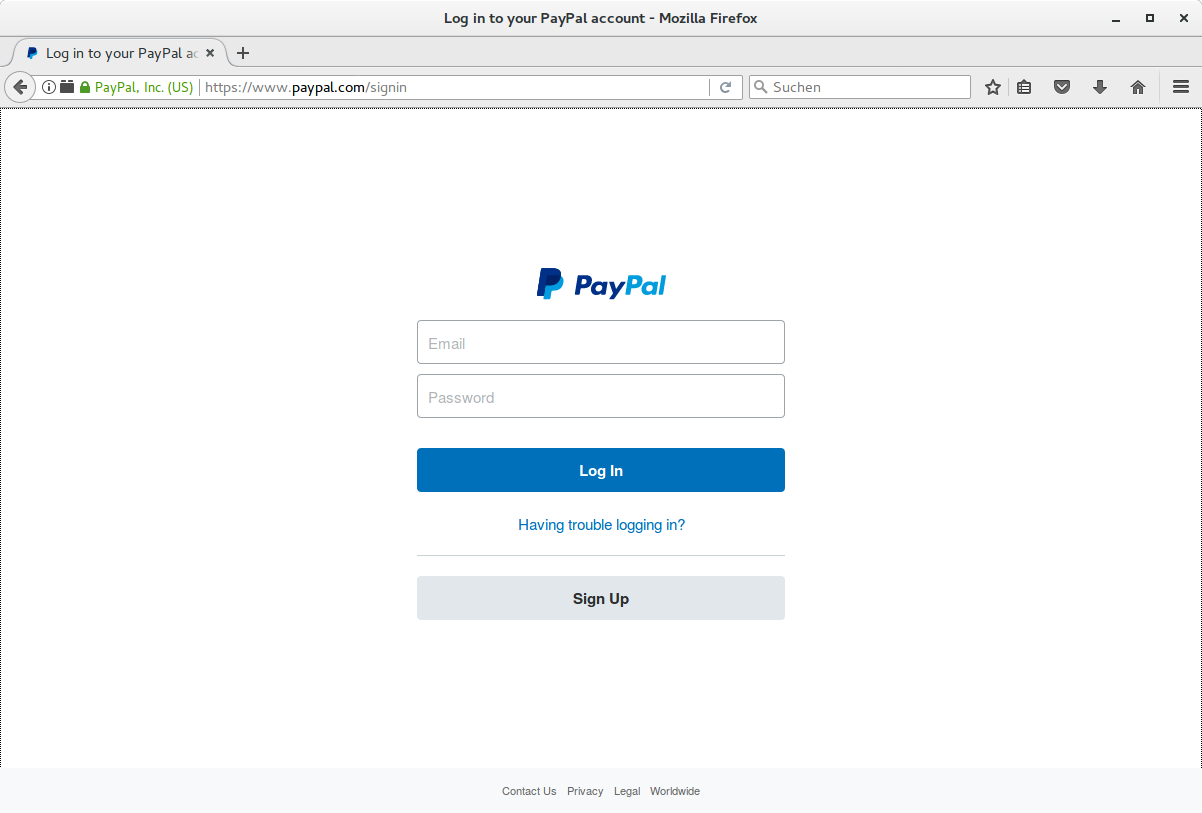
\includegraphics[width=15cm]{images/paypal-original-site}
  \caption{PayPal Original Webseite}
  \label{fig:paypal-original-site}
\end{figure}

Das Vorgehen im vorausgegangen Beispiel ist sehr typisch für Phishing-Angriffe und kann deshalb auf sehr viele andere Seiten übertragen werden.

\todo{Samuel}